Distributed file systems provide a unified interface to applications and clients,
yet they consist of a number of disks and servers.
%
Partitioning files and put them on separate disks and servers is a common practice,
because this approach provides aggregated storage capacity and bandwidth.
%
This section surveys partitioning strategies adopted by the three file systems,
and disscuss the advantages and disadvantages of them.


\subsection{Chunks in Google File System}
\label{sec:partition_gfs}
%
\begin{figure}
\centering
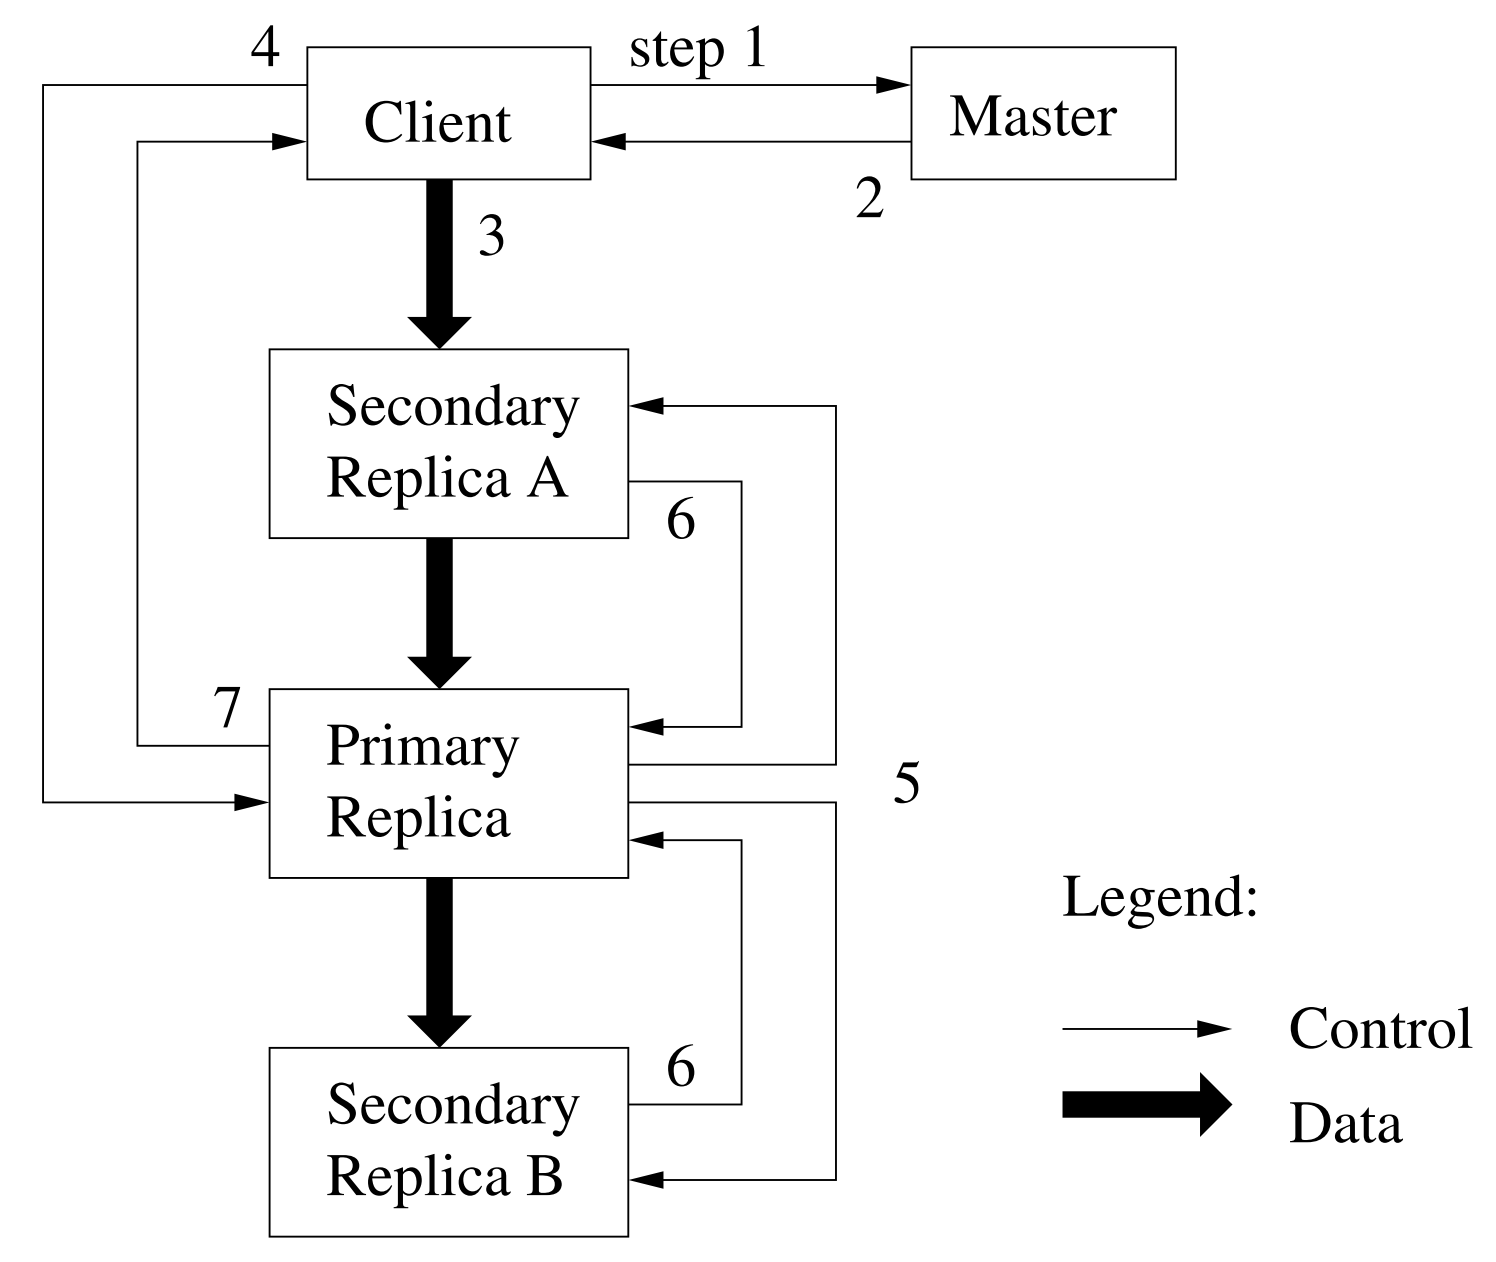
\includegraphics[width=0.95\columnwidth]{image/gfs_data_flow.png}
\caption{GFS data flow}
\label{fig:gfs_data_flow}
\end{figure}
%
Google File System partition data into chunks~\cite{ghemawat2003google}.
%
Each chunk has a relatively big size: 64MB.
%
This relatively large chunk size has a few benefits:
%
\begin{enumerate}
\item it reduces clients' need to interact with the master node, because reads 
	and writes on the same chunk require only one initial request to the master;
\item it reduces the network overhead by keeping a persistent TCP connection to
	the chunkserver over a longer time, rather than establishing multiple 
	connections;
\item it reduces the size of metadata saved on the master, which helps improve
	the overall system performance. 
\end{enumerate}

Each chunk has replicas across the entire GFS.
%
By default, there are three replicas.
%
The benefit of replicas is two-fold.
%
First, this redundancy provides reliability. 
%
In case of one or even two replicas fail, the data is still safe.
%
Second, replicas located in different servers provide more flexible 
access to clients.
%
When reading data, a client reads from a certain replica that is 
1) has less network delays to the client; and
2) resides on a server with less load.

\subsubsection{Data Flow in GFS}
The chunk replication mechanism of GFS requires careful handling 
when writing data onto the disk.
%
Specifically, writing to multiple replicas should not take multiple times longer.
%
GFS uses two approaches to speed up data write on multiple replicas:
%
\begin{enumerate}
\item decouple the expensive data flow and inexpensive control flow;
\item data flows in a pipelined fashion along a chain of chunkservers.
\end{enumerate}

Data flow starts from the client who has a write task, following a linear chain
of chunkservers.
%
To make best use of the machine's network bandwidth, each machine forwards the
data to the ``closest" machine in the network topology that has not received it.
%
This forwarding step happens immediately after a chunkserver receives some data.
%
Each chunkserver puts received data in the buffer without immediate commit;
rather, it only commits until all chunkservers finish receiving data, and 
receives a commit instruction.

Control flow communicates different information between different nodes:
\begin{enumerate}
\item master tells client which chunkserver holds the current lease for 
	the chunk and the locations of the other replicas;
\item client sends a commit instruction to the ``primary" of the multiple
	chunkservers when all chunkservers finish receiving data;
\item the ``primary" chunkserver sends commit instruction to all the secondary
	chunkservers; and
\item the ``primary" chunkserver replies to the client that all replicas are 
	successfully committed.
\end{enumerate}

The benefit of the decoupling of data flow and control flow is that control 
flows become light-weighted so that they are more tolerant to failures 
of any kind.
%
Data flow is heavy-weighted, but this operation is relatively simple:
it happens in an ``all or nothing" fashion.
%
Data is committed only after all chunkservers successfully
receive the full data to write.
%
This data flow paradigm is shown in Figure~\ref{fig:gfs_data_flow}.



\subsection{Stripes in GPFS}
\label{sec:stripe_gpfs}
%
\begin{figure}
\centering
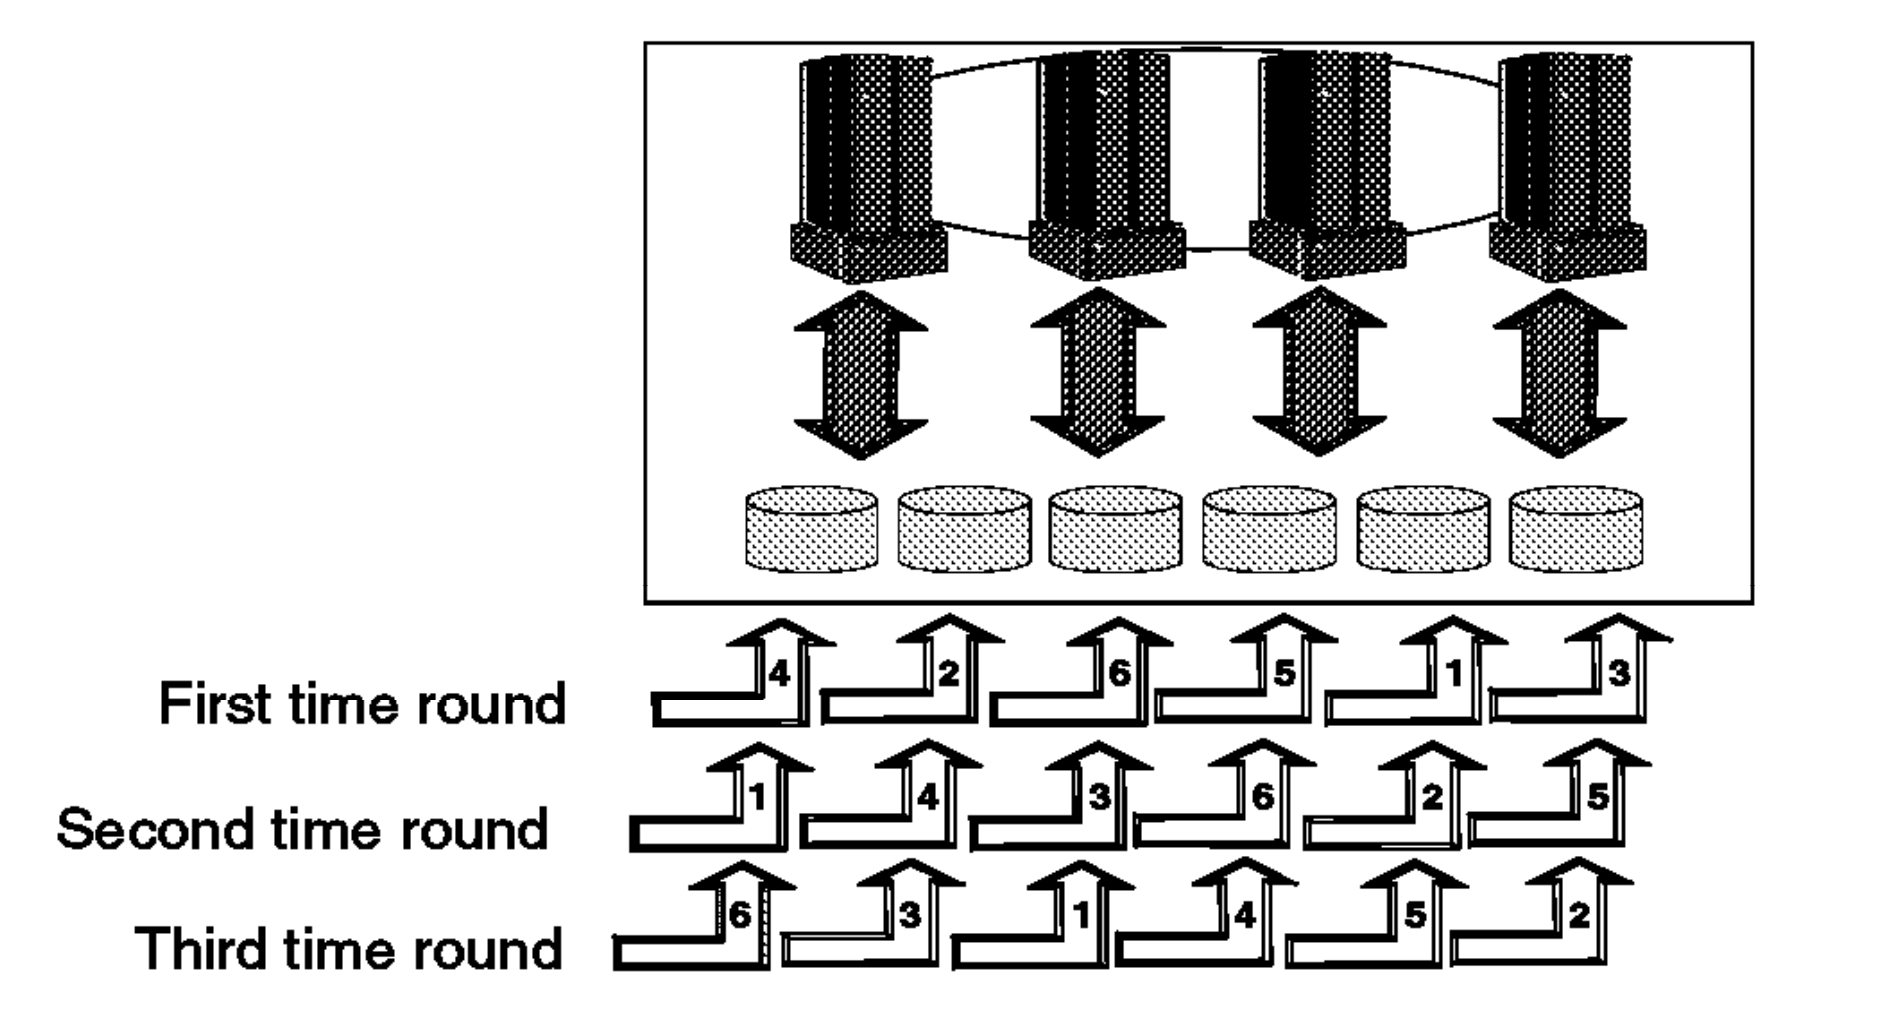
\includegraphics[width=1\columnwidth]{image/balancedrandom.png}
\caption{Balanced Random striping. Disk order is not enforced from the 
	first to the second to the third round, but the overall load across
	multiple disks is kept balanced.}
\label{fig:balancedrandom}
\end{figure}
%
\begin{figure}
\centering
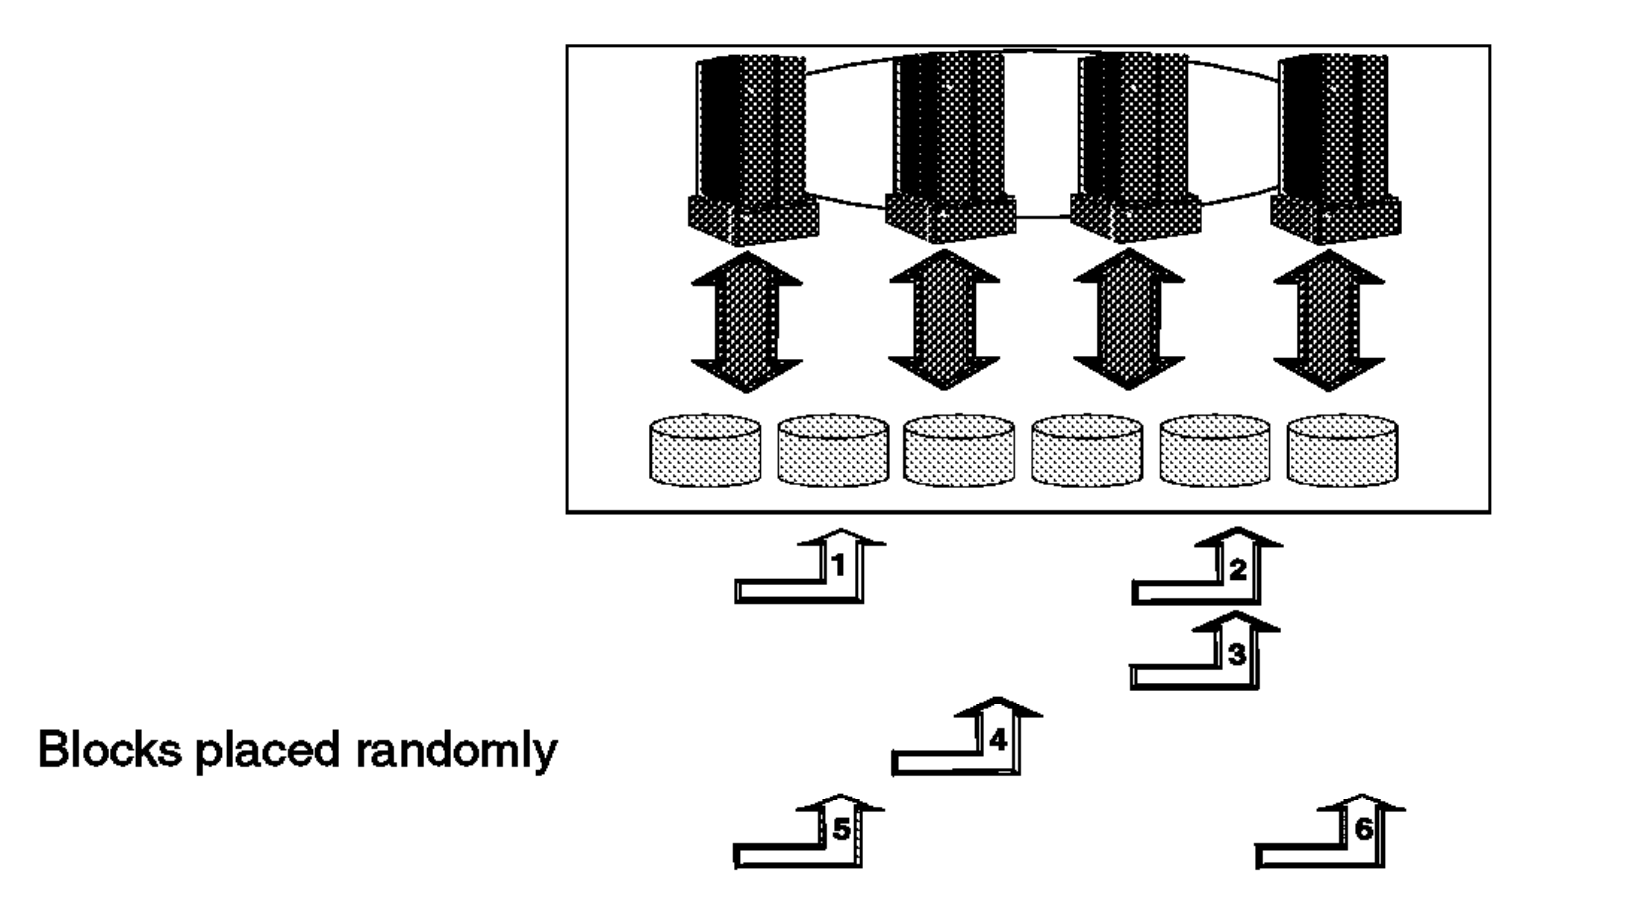
\includegraphics[width=1\columnwidth]{image/random.png}
\caption{Random striping. Each data block is randomly placed on a 
		disk. Load balance is not ensured by this striping scheme.}
\label{fig:random}
\end{figure}
%
%
GPFS adopts a decentralized architecture (Section~\ref{sec:archi_gpfs}),
so files are striped across all disks in the file 
system~\cite{Schmuck2002,barkes1998gpfs}.
%
Each file is divided into equal sized blocks, and consecutive blocks are 
placed on different disks in a round-robin fashion by default.
%
The choice of block size is very different from that of GFS though: 
GPFS allows  block size between 16KB and 1MB, with 256KB being the 
default size (compared to the 64MB chunk size by GFS).

To ensure maximum parallelism when reading a large file, GPFS issues 
I/O requests in parallel to as many disks as necessary.
%
Similarly, data buffers that are no longer being accessed are written 
to disk in parallel.
%
This practice is enabled by the property of GPFS that all nodes in the cluster
have equal access to all disks~\ref{sec:archi_gpfs};
it also achieves reading or writing data from/to a single file at the 
aggregate data rate supported by the underlying disk subsystem and 
interconnection fabric.

The round-robin fashion to place file blocks requires equal size and performance
among all disks to achieve best disk utilization and performance.
%
A non-uniform disk configuration requires a trade-off between throughput and space
utilization: maximizing space utilization means placing more data on larger disks, 
but this reduces total throughput.
%
GPFS allows the administrator to make this trade-off by specifying
whether to balance data placement for throughput or space utilization.

Besides round-robin, GPFS provides another two striping options, mainly
to ease the strict disk order enforced by round-robin option:
1) balanced random striping, and
2) random striping.
%
Round-robin achieves best performance but it also suffers from the longest
time to re-stripe the files in any unexpected event.
%
Balanced random differs from RoundRobin in that each data 
block is written to a disk selected randomly. 
%
However, the same as in the round-robin  method, the same disk is not 
selected until all the disks within the stripe group have been used.
%
Figure~\ref{fig:balancedrandom} illustrates this striping method.
%
With random striping, each block of data is written on a disk 
selected randomly. 
%
No surprise, this method does not assure that the traffic will be 
balanced among all the disks.
%
Balanced random and random striping approaches are usually used when 
re-striping is expected to happen frequently.



\subsection{Stripes in Lustre}
\label{sec:stripe_Lustre}
%
Striping in Lustre follows a similar pattern as it is in GPFS, in that files 
are divided into multiple stripes to achieve aggregated performance.
%
This section we address two major differences between them though.

The first difference is that Lustre supports locating file blocks based on 
the available free space on each object storage target (OST)
\cite{Schwan2003,braamlustre}.
%
More specifically, when the free space across OSTs differs by more than 
a specific amount (17\% by default), the metadata server (MDS) then uses 
weighted random allocations with a preference for allocating objects on OSTs 
with more free space.
%
This can reduce I/O performance until space usage is rebalanced again.

The second difference is that Lustre uses a large block size than GPFS.
%
In contrast to the 16KB to 1MB in GPFS, Lustre supports a 512KB to 4GB 
block size.


\subsection{Discussion on Partitioning Schemes}
\label{sec:discuss_partitioning}
%
Among the three surveyed file systems, there is a big difference regarding 
the file access patterns between GFS and the other two: GPFS and Lustre.
%
In GFS, most files are mutated by appending new data rather than 
overwriting existing data. 
%
A much larger block size helps to reduce the overload of asking and exchanging
the file locks. 
%
While in GPFS and Lustre, most file operations are normal creating and reading
tasks, resulting in the design choice of smaller block sizes.

GFS also puts more emphasis on data replications. 
%
Particularly, GFS itself manages the replications.
%
The GPFS and Lustre do not focus on data replications though.
%
They mostly use Redundant Array of Independent Disks (RAID) and leave
the data replication job to RAID.
 



